\section{Evaluation}
\label{ch:eval}

In this chapter, we conduct evaluations to our collected data.
The data is collected from 21 subjects, and 189 clickstream data are collected in total. 
Each clickstream contains action-level data with a stay duration
of a specific page, for instance, we still collect an URL as a step of clickstream 
if a participant uses back button rollback to a previous visited page without requesting server. 
A clickstream also has a subjective difficulty score from questionaire (shown in Appendix \ref{appendix:b}) 
after the completion of each task.

\subsection{Subjective Task Difficulty}

This section discusses the subjective task difficulty qualitatively and quantitatively.
Figure \ref{fig:difficulty} illustrates a normalized (raw scores are listed in 
Appendix \ref{appendix:c} Table \ref{table:diff-raw}) subjective difficulty score 
with respect to all tasks.

\begin{figure}[H]
    \centering
    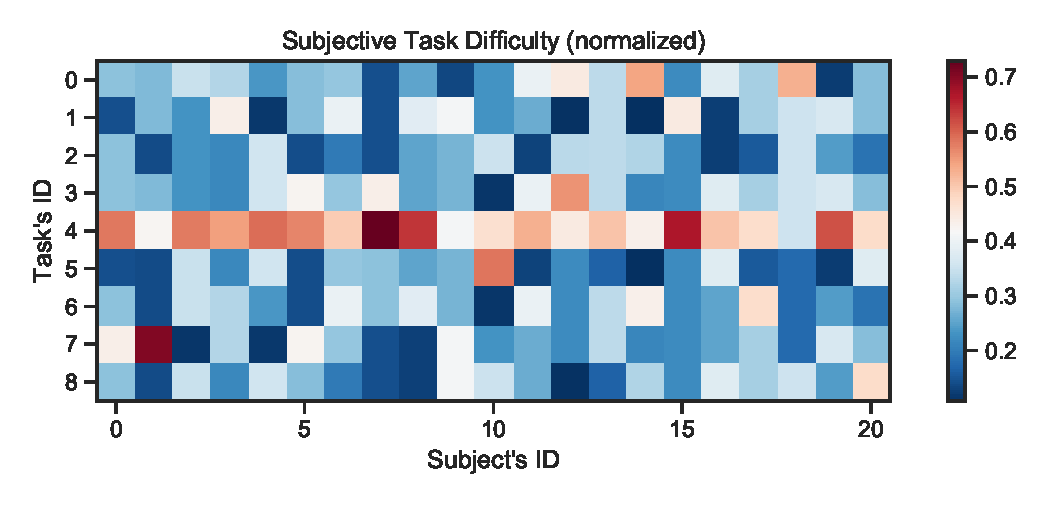
\includegraphics[width=0.7\textwidth]{figures/difficulty}
    \caption{Subjective difficulty score: each column indicates an individual subject and
    each row indicates a browsing task. Tasks from 0 to 8 represent Amazon Goal Oriented Task,
    Amazon Fuzzy Task, Amazon Exploring Task; Medium Goal Oriented Task, Medium Fuzzy Task,
    Medium Exploring Task, Dribbble Goal Oriented Task, Dribbble Fuzzy Task and Dribbble Exploring Task
    respectively.
    From this heat map, we clearly observes Medium Fuzzy Task is the most difficulty task
    according to the subjects voted subjective difficulty, a Mann-Whitney U significant 
    test justifies this observation.}
    \label{fig:difficulty}
\end{figure}

To generalize the task difficulty, the null hypothesis ($H_0$): the difficulty of fuzzy task is not greater
than exploring task and alternative hypothesis ($H_1$): the difficulty of fuzzy task is greater than
exploring task. We conduct non-parametric one-tailed Mann-Whitney U test \cite{mann1947test}, 
under null hypothesis, $p=2.54\times 10^{-5} < 0.05$, reject $H_0$.
Similarly, we compare difficulty score on goal oriented task and exploring task (with corresponding hypothesis, 
$p=0.00534 < 0.05$), difficulty score on fuzzy task and goal oriented task (with corresponding hypothesis, 
$p=0.0145 < 0.05$), all rejects $H_0$. Therefore we concludes the task difficulty is ordered
as follows: \emph{difficulty of fuzzy task $>$ difficulty of goal oriented task $>$ difficulty of exploring task},
which means exploring tasks have lower effort in clickstream, and effort of doing fuzzy task gains highest effort.

\subsection{Browsing Behavior Classification}

As discussed in Section \ref{sec:task-design}, we described three type of browsing behavior. 
In this section, we provides two type of evaluations to interpret the browsing behavior classification.

First, we evaluate the indication of general features browsing behavior,
features including difficulty of task, number of actions in a clickstream as well as the total stay duration in a clickstream.
Then we implements our action path model by using the action-level clickstream data and stay duration of each page,
which was described in Section \ref{sec:recurrent-unit} and \ref{sec:mark-interpretation}.

\subsubsection{Interpretation based on General Features}
\label{sec:inter-general-feature}

As a baseline of our classification performance, we use the \textbf{completion efficiency}, 
\textbf{total time duration of a task} 
as well as \textbf{total number of actions of a task} as the three features for
browsing behavior classification.

Note that the completion efficiency is defined by the shortest path of entire clickstream,
 and the completion efficiency cannot can only be determined if and only if the clickstream
 is given, in a sense, it carries a latent information of browsing behavior.

We applied gird-search on support vector machine (SVM) with polynomial kernel,
the best classification precision is 0.53 ($C=4.5, \gamma = 1.5$),
and the micro average F1 score is also 0.53, which is better than random (0.33).

\begin{figure}[H]
    \centering

    \begin{subfigure}[b]{0.45\textwidth}
        \includegraphics[width=1\textwidth]{figures/tsne-amazon}
        \caption{}
        \label{fig:tsne-amazon}
    \end{subfigure}
    \begin{subfigure}[b]{0.45\textwidth}
        \includegraphics[width=1\textwidth]{figures/2d-eff-dur-amazon}
        \caption{}
        \label{fig:2d-eff-dur-amazon}
    \end{subfigure}
    \begin{subfigure}[b]{0.45\textwidth}
        \includegraphics[width=1\textwidth]{figures/2d-eff-len-amazon}
        \caption{}
        \label{fig:2d-eff-len-amazon}
    \end{subfigure}
    \begin{subfigure}[b]{0.45\textwidth}
        \includegraphics[width=1\textwidth]{figures/2d-len-dur-amazon}
        \caption{}
        \label{fig:2d-len-dur-amazon}
    \end{subfigure}

    \caption{In these figures, \ref{fig:tsne-amazon} shows the t-SNE projection
    of completion efficiency, total time duration and number of actions for three different behavior;
    \ref{fig:2d-eff-dur-amazon} is a 2D comparasion of using completion efficiency and total time duration;
    \ref{fig:2d-eff-len-amazon} provides a 2D comparasion of using completion efficiency and number of actions;
    \ref{fig:2d-len-dur-amazon} shows a 2D comparasion of using number of actions and total time duration.
    From t-SNE visualization, we observed that exploring tasks tend to centralized on the right and goal-oriented
    tasks and fuzzy tasks tend to centralized on the left, which indicates that exploring behaviors tend to classifiable
    comparing to other two behaviors. According the rest of feature comparasion visualizations, the completion effeciency and total time duration
    contributes more on interpret exploring behavior, and the number of actions tent to
    contributes more on interpret goal-oriented task.}
    \label{fig:general-amazon}
\end{figure}

To understand the meaning of classification, we also applies a randomized decision tree
that gives the importance of the used features: \emph{total time duration and number of actions
of a task is more important than our self defined completion efficiency.}

More specifically, we applies one-tailed Mann-Whitney U test for each of the features,
for instance the null hypothesis ($H_0$): the completion efficiency of goal-oriented task 
is not greater than exploring task, we have $p = 0.0019 < 0.05$ reject $H_0$, which means
the completion efficiency of goal-oriented task is significant efficient than than exploring task.

Similarly, we conduct the significant test with similar hypothesis 
to all comparable combinations as showed in Table \ref{table:sig-test-efficiency}, \ref{table:sig-test-duration}, and \ref{table:sig-test-actions}.

\begin{table}[H]
    \small
    \centering
    \caption{One-tailed significant test for completion efficiency in different browsing behaviors.
    The null hypothesis in this table, for instance, completion efficiency of fuzzy task
    is \emph{not} significant efficient than goal-oriented task, the result $p=0.45>0.05$ which means
    accept $H0$. Similar to others.}
        \begin{tabular}{cccc}
            \toprule
              v.s.             & efficiency goal & efficiency fuzzy & efficiency explore \\
            efficiency goal    & N/A             & reject           & reject             \\
            efficiency fuzzy   & accept          & N/A              & reject             \\
            efficiency explore & accept          & accept           & N/A                \\
            \bottomrule
        \end{tabular}
        \label{table:sig-test-efficiency}
\end{table}

\begin{table}[H]
    \small
    \centering
    \caption{One-tailed significant test for total stay duration of a task in different browsing behaviors.
    The null hypothesis in this table, for instance, total stay duration of fuzzy task
    is \emph{not} significant stay longer than goal-oriented task, the result $p=0.41>0.05$ which means
    accept $H0$. Similar to others.}
        \begin{tabular}{cccc}
            \toprule
              v.s.             & duration goal & duration fuzzy & duration explore \\
            duration goal      & N/A & reject & reject \\
            duration fuzzy     & accept & N/A & reject \\
            duration explore   & accept & accept & N/A \\
            \bottomrule
        \end{tabular}
        \label{table:sig-test-duration}
\end{table}

\begin{table}[H]
    \small
    \centering
    \caption{One-tailed significant test for total number of actions of a task in different browsing behaviors.
    The null hypothesis in this table, for instance, total number of actions of fuzzy task
    is \emph{not} significant performs more actions than goal-oriented task, the result $p=0.019<0.05$ which means
    reject $H0$. Similar to others.}
        \begin{tabular}{cccc}
            \toprule
              v.s.             & actions goal & actions fuzzy & actions explore \\
              actions goal      & N/A & accept & reject \\
              actions fuzzy     & reject & N/A & accept \\
              actions explore   & accept & reject & N/A \\
            \bottomrule
        \end{tabular}
        \label{table:sig-test-actions}
\end{table}

As conclusions, we summarized that:

\begin{itemize}
    \item \textbf{Completion efficiency}: the completion efficiency of goal-oriented and fuzzy behavior is significant efficient than exploring behavior;
    \item \textbf{Number of actions}: the number of actions of goal-oriented behavior is significant lower than fuzzy and exploring behaviors.
    \item \textbf{Total stay duration}: the total stay duration of explroing behavior is significant higher than goal-oriented and fuzzy behaviors.
\end{itemize}

Furthermore, the completion efficiency and total stay duration are the more important than others for indication of exploring behavior,
and number of actions are more important than others for indication of goal-oriented behavior.

\subsubsection{Intepretation based on Action Path}
\label{sec:inter-action-path}

To use full capacity of our data, this section uses the entire clickstream and its corresponding
page-level stay duration as input, three ending mark (<EOA\_GOAL>, <EOA\_FUZZY>, and <EOA\_EXPLORE>) 
as classification outputs, and then implements a single GRU layer action path model 
to classify the three type of browsing behaviors.

Our training parameters are: 
The GRU latent dimension is 10, training process feeds 132 clickstreams as training data,
38 clickstreams as validation, then 
propagates 500 epochs with batch size of 32. In the training process, we use Adam optimizer,
 categorical corss-entropy loss as well as L1 and L2 regularizer with early stopping.

In the end of training, we evaluates 19 clickstreams as testing dataset and 
archieved \textbf{100.00\% accuracy} of browsing behaviors classification.

\begin{figure}[H]
    \centering
    \includegraphics[width=0.55\textwidth]{figures/class-loss}
    \caption{Categorical Cross-Entropy Validation loss curve while 500 epoches. 
    The curves indicates the training process is not an overfitting since the loss is not increasing.}
    \label{fig:class-loss}
\end{figure}

One can observed that the training process is not an overfit, and the validation loss is 
still not increase after 500 epoches, thus, single GRU layer action path model 
remains a large expressive generalization performance 
(100\% accuate for three browsing behavior classification), therefore
we expect to collect more data to verify whether the model applicable to a large dataset.

In addition, the action path model feeds the entire clickstream and time duration as inputs, 
therfore the entire clickstream contains informations regarding the number of actions
as well as completion effeciency and more latent informations. 
Consequently, we conclude that the model works
\emph{perfectly on the classification of three different browsing behavior}. 
Since our experiment is only designed for three type of behavior, and the learning curve
shows the model still has capacity and generalization ability to 
classify more precise categories of browsing behavior, a future investigation on
more categories may be worthwhile.

\subsection{Optimal Action Path Context}

This section we evaluates our model with limited action path context, where the feeding action path
are limited based on a split ratio. 
For instance, if a split ratio is 0.8 then we feed 80\% of an action path into the model, 
then predict the rest of 20\% actions. Figure \ref{fig:acc} illustrates the best accuracy 
we archieved from a single layer action path model when use with different split ratio.

\begin{figure}[H]
    \centering
    \includegraphics[width=0.7\textwidth]{figures/acc}
    \caption{Prediction accuracy with limited context of input. This figure illustrates, wih more context of clickstream
    known to the action path model, more information to the model, and therefore much higher accuracy we can archieve.
    The accuracy we evaluated here is a greedy search accuracy, and thus higher than 25\% of prediction accurate is acceptable,
    i.e. a quater of future movements are predicted correctly.
    On the right side of the figure, we archieved >60\% accuracy of 3 to 5 future steps prediction.
    Classification is a special case in this figure where split ratio is equal to 0.99.}
    \label{fig:acc}
\end{figure}

This figure illustrates, wih more context of clickstream
feeds into the action path model, the model receive more informations of the clickstream, 
and therefore much higher accuracy we can archieve for prediction.
The accuracy we evaluated here is a greedy search accuracy, which performs element-wise comparasion
between predicted clickstream and ground trueth clickstream, and the accuracy is the number of
corrected predictions divided by total number of prediction steps.

An accuracy that higher than 25\% is acceptable in our prediction task, since it indicates
a quater of future movements are predicted correctly.
On the right side of the figure, we archieved >60\% accuracy of 3 to 5 future steps prediction.

\begin{figure}[H]
    \centering
    \includegraphics[width=0.55\textwidth]{figures/loss2}
    \caption{Validation loss curve when split ratio is 0.97. The loss indicates
    the model may be reparameterized while training and archieve better performance
    for predictions.}
    \label{fig:loss}
\end{figure}

Note that the prediction is still not an overfitting to the dataset. Figure \ref{fig:loss}
illustrates the loss curve while training over 1500 epochs with 3 steps of prediction (split ratio 0.97).
The loss starts increase after almost 200 epochs, which may be represent to overfitting,
nevertheless, one can observe that the loss decreases down to similar level of early training 
and archieved a better performance (almost 60.0\% of precision) than previous, which indicates
the training process may reparameterize the action path model while training and archieve better performance
for predictions.

\subsection{Action Path Visualization}

This section visualizes the actual action path of users and discusses the behavior qualitatively.
In total, we collected 189 clickstream, which is not possible to illustrate all of them
in the thesis, we selected three typical clickstreams to discuss and provided a visualization tool
(see Appendix \ref{appendix:a}) to help readers to explore them.

\subsubsection{Individual Common Patterns}

The first pattern one can observe from the goal-oriented task clickstream is ``cluster''.
In Figure \ref{fig:vis-goal1} and \ref{fig:vis-goal2}, the visualization shows different clustered intents in
Amazon's goal-oriented task. We can easily discriminate the user browsing for 
different intent in different cluster, and then finally went to the cart without
backtracking.

Beyound the cluster pattern, we also observes ``hesitation'' pattern in goal-oriented tasks
where a short child path branch from its parent node in each intent cluster, e.g. node
4, 8, 14 in Figure \ref{fig:vis-goal1} and node 5, 16 in Figure \ref{fig:vis-goal2},
which suggests ``hesitation'' is a pattern that more often appears in goal-oriented task
within a ``cluster''.

\begin{figure}
    \centering
    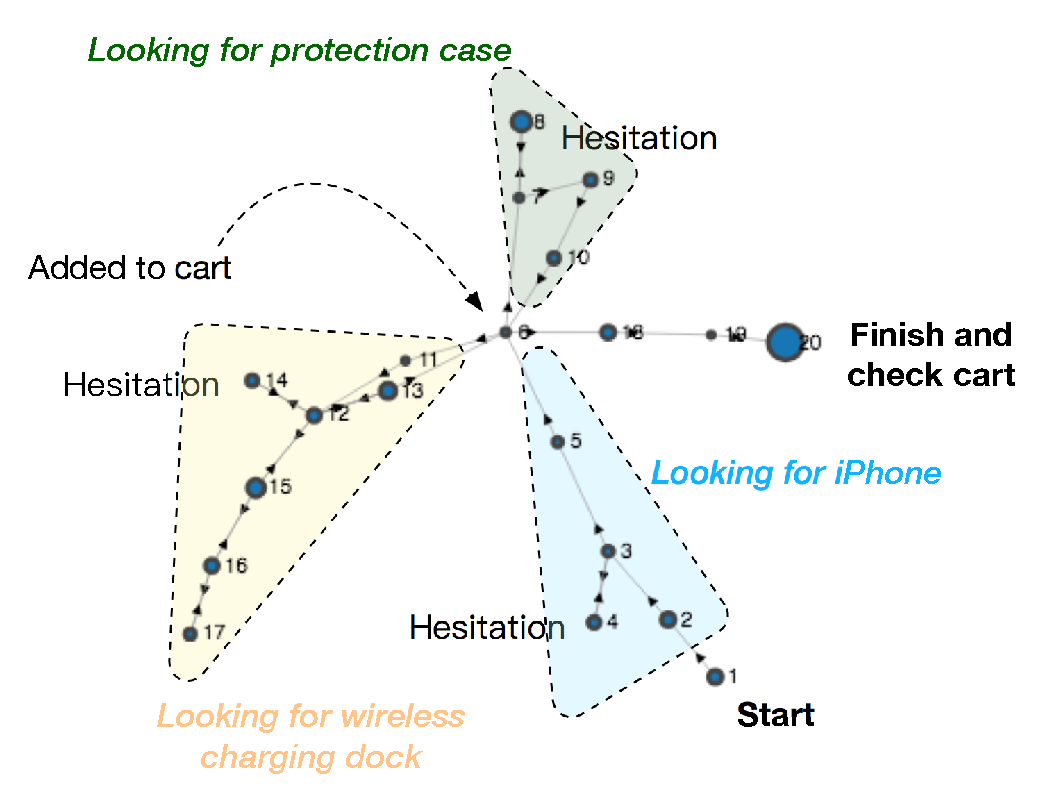
\includegraphics[width=0.55\textwidth]{figures/vis-goal1}
    \caption{Validation loss curve when split ratio is 0.97. The loss indicates
    the model may be reparameterized while training and archieve better performance
    for predictions.}
    \label{fig:vis-goal1}
\end{figure}

\begin{figure}
    \centering
    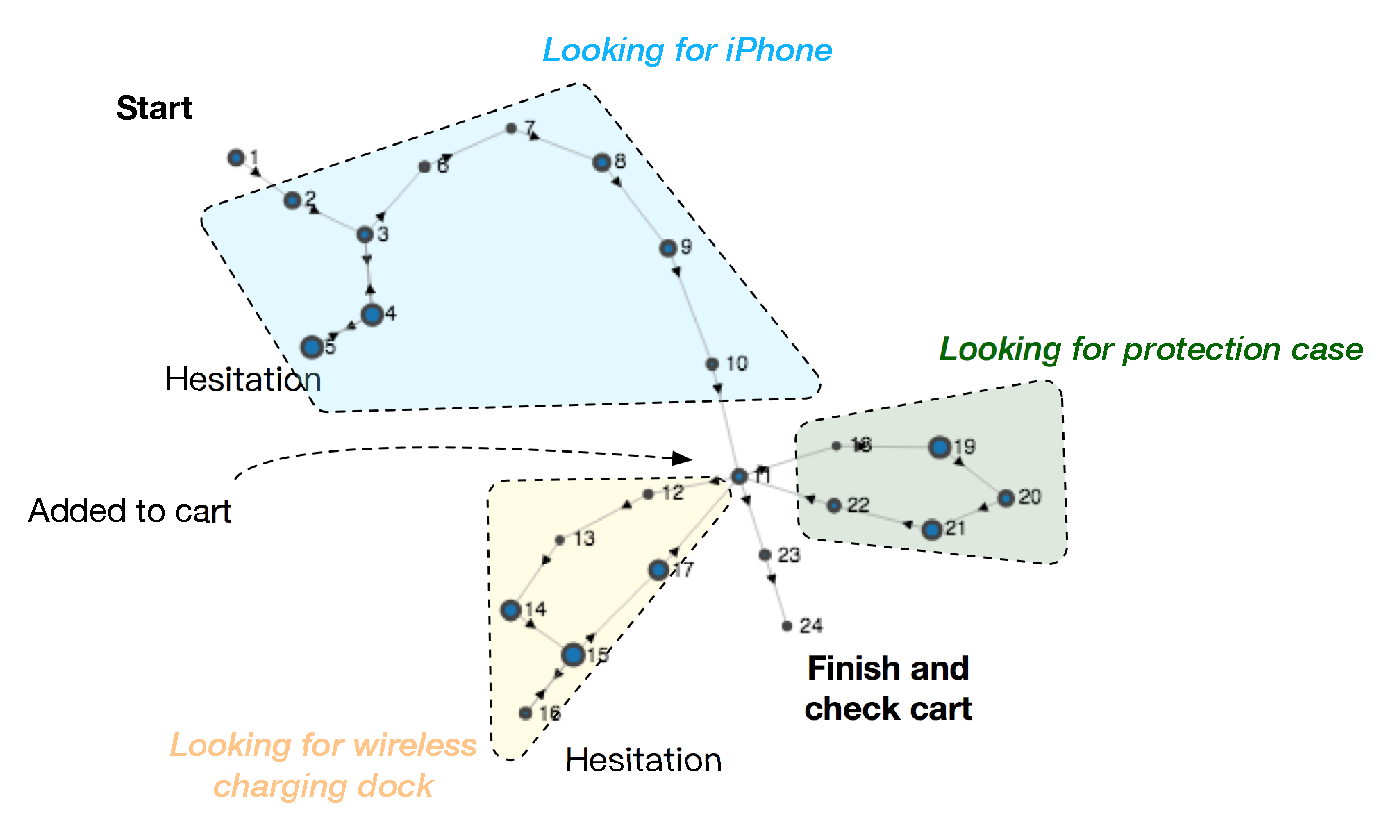
\includegraphics[width=0.55\textwidth]{figures/vis-goal2}
    \caption{Validation loss curve when split ratio is 0.97. The loss indicates
    the model may be reparameterized while training and archieve better performance
    for predictions.}
    \label{fig:vis-goal2}
\end{figure}

Similarly, in fuzzy and exploring task, we observed two common pattern ``ring'' and ``star''
pattern is more often to appear in fuzzy and exploring tasks.

\begin{figure}[H]
    \centering
    \begin{subfigure}[b]{0.60\textwidth}
        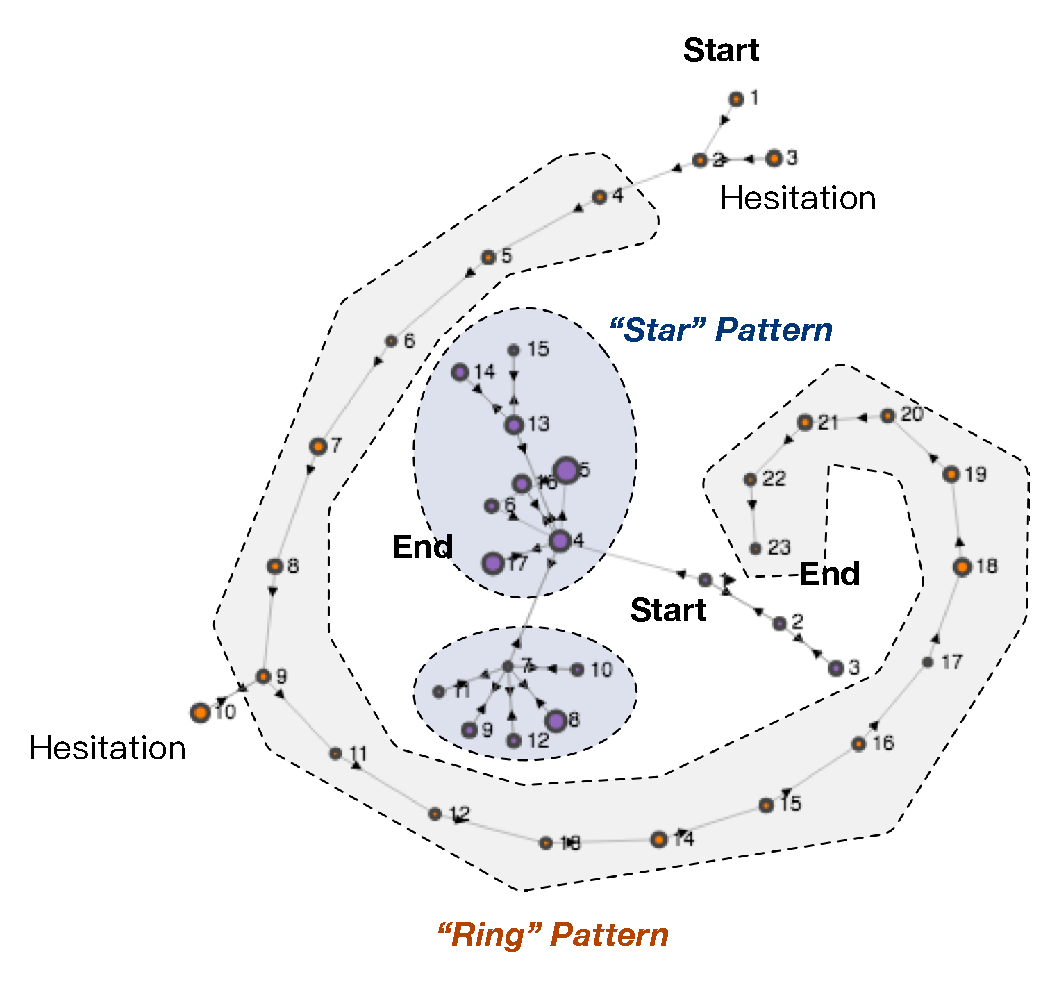
\includegraphics[width=1\textwidth]{figures/vis-patterns1}
        \caption{}
        \label{fig:vis-fuzzy-explore1}
    \end{subfigure}
    \begin{subfigure}[b]{0.60\textwidth}
        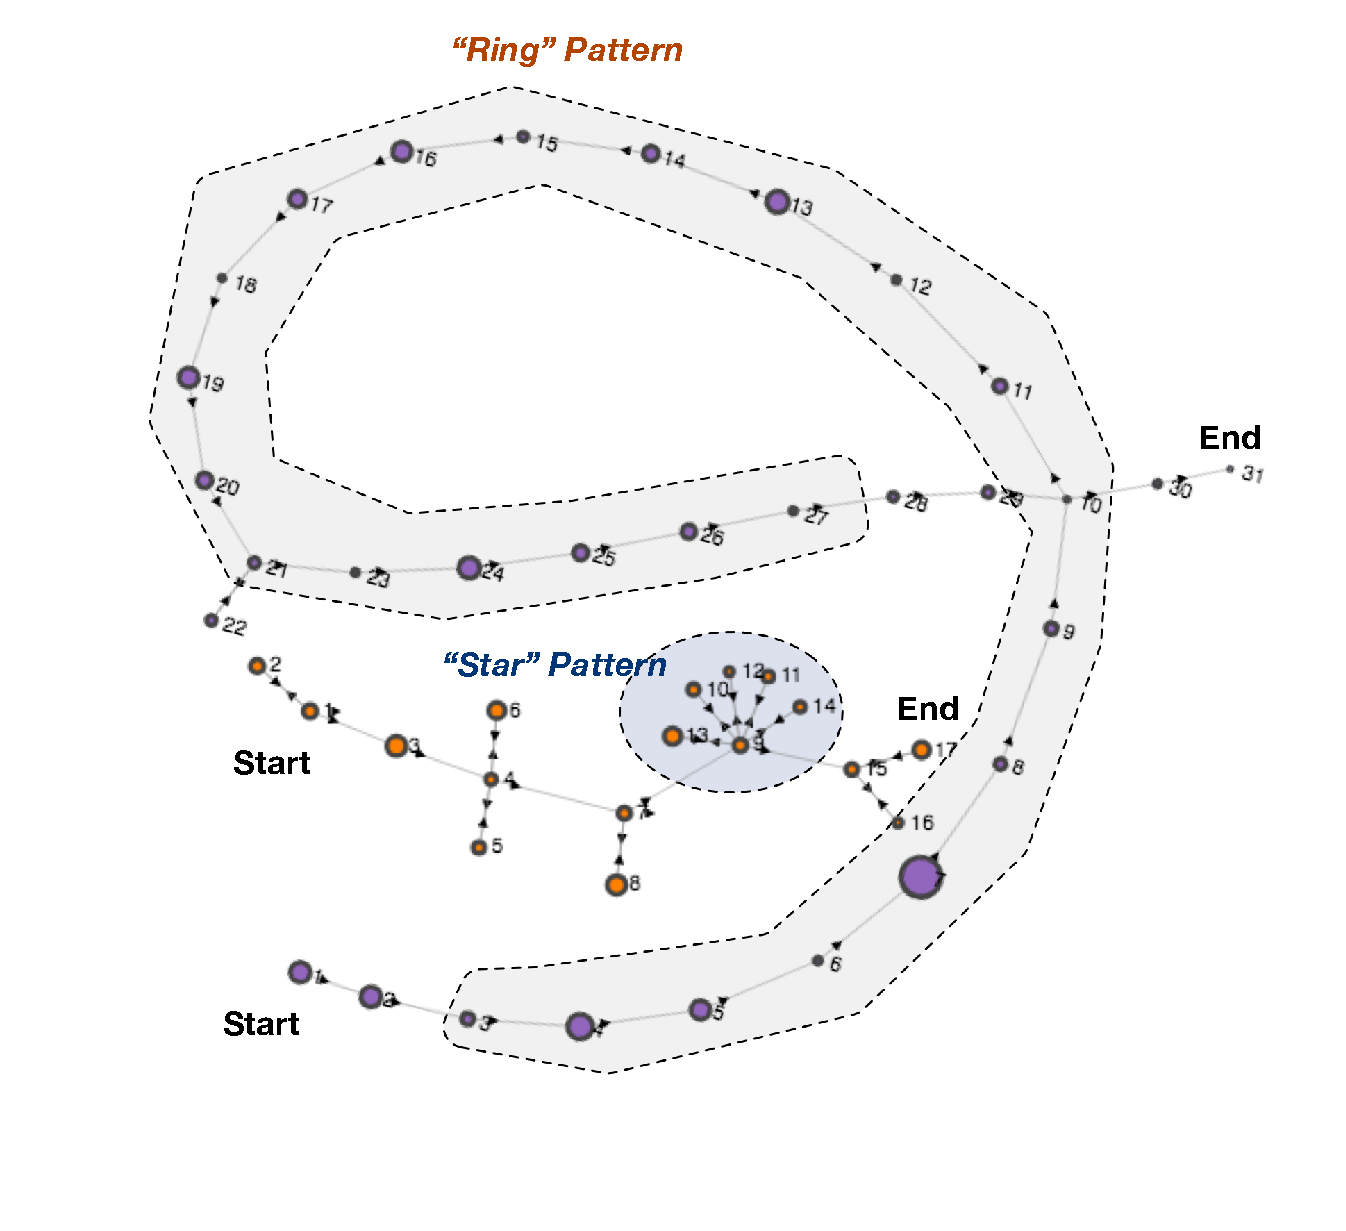
\includegraphics[width=1\textwidth]{figures/vis-patterns2}
        \caption{}
        \label{fig:vis-fuzzy-explore2}
    \end{subfigure}
    \caption{TODO:}
    \label{fig:vis-fuzzy-explore}
\end{figure}

\subsubsection{Cross-user Overlap Patterns}

\begin{figure}[H]
    \centering

    \begin{subfigure}[b]{0.60\textwidth}
        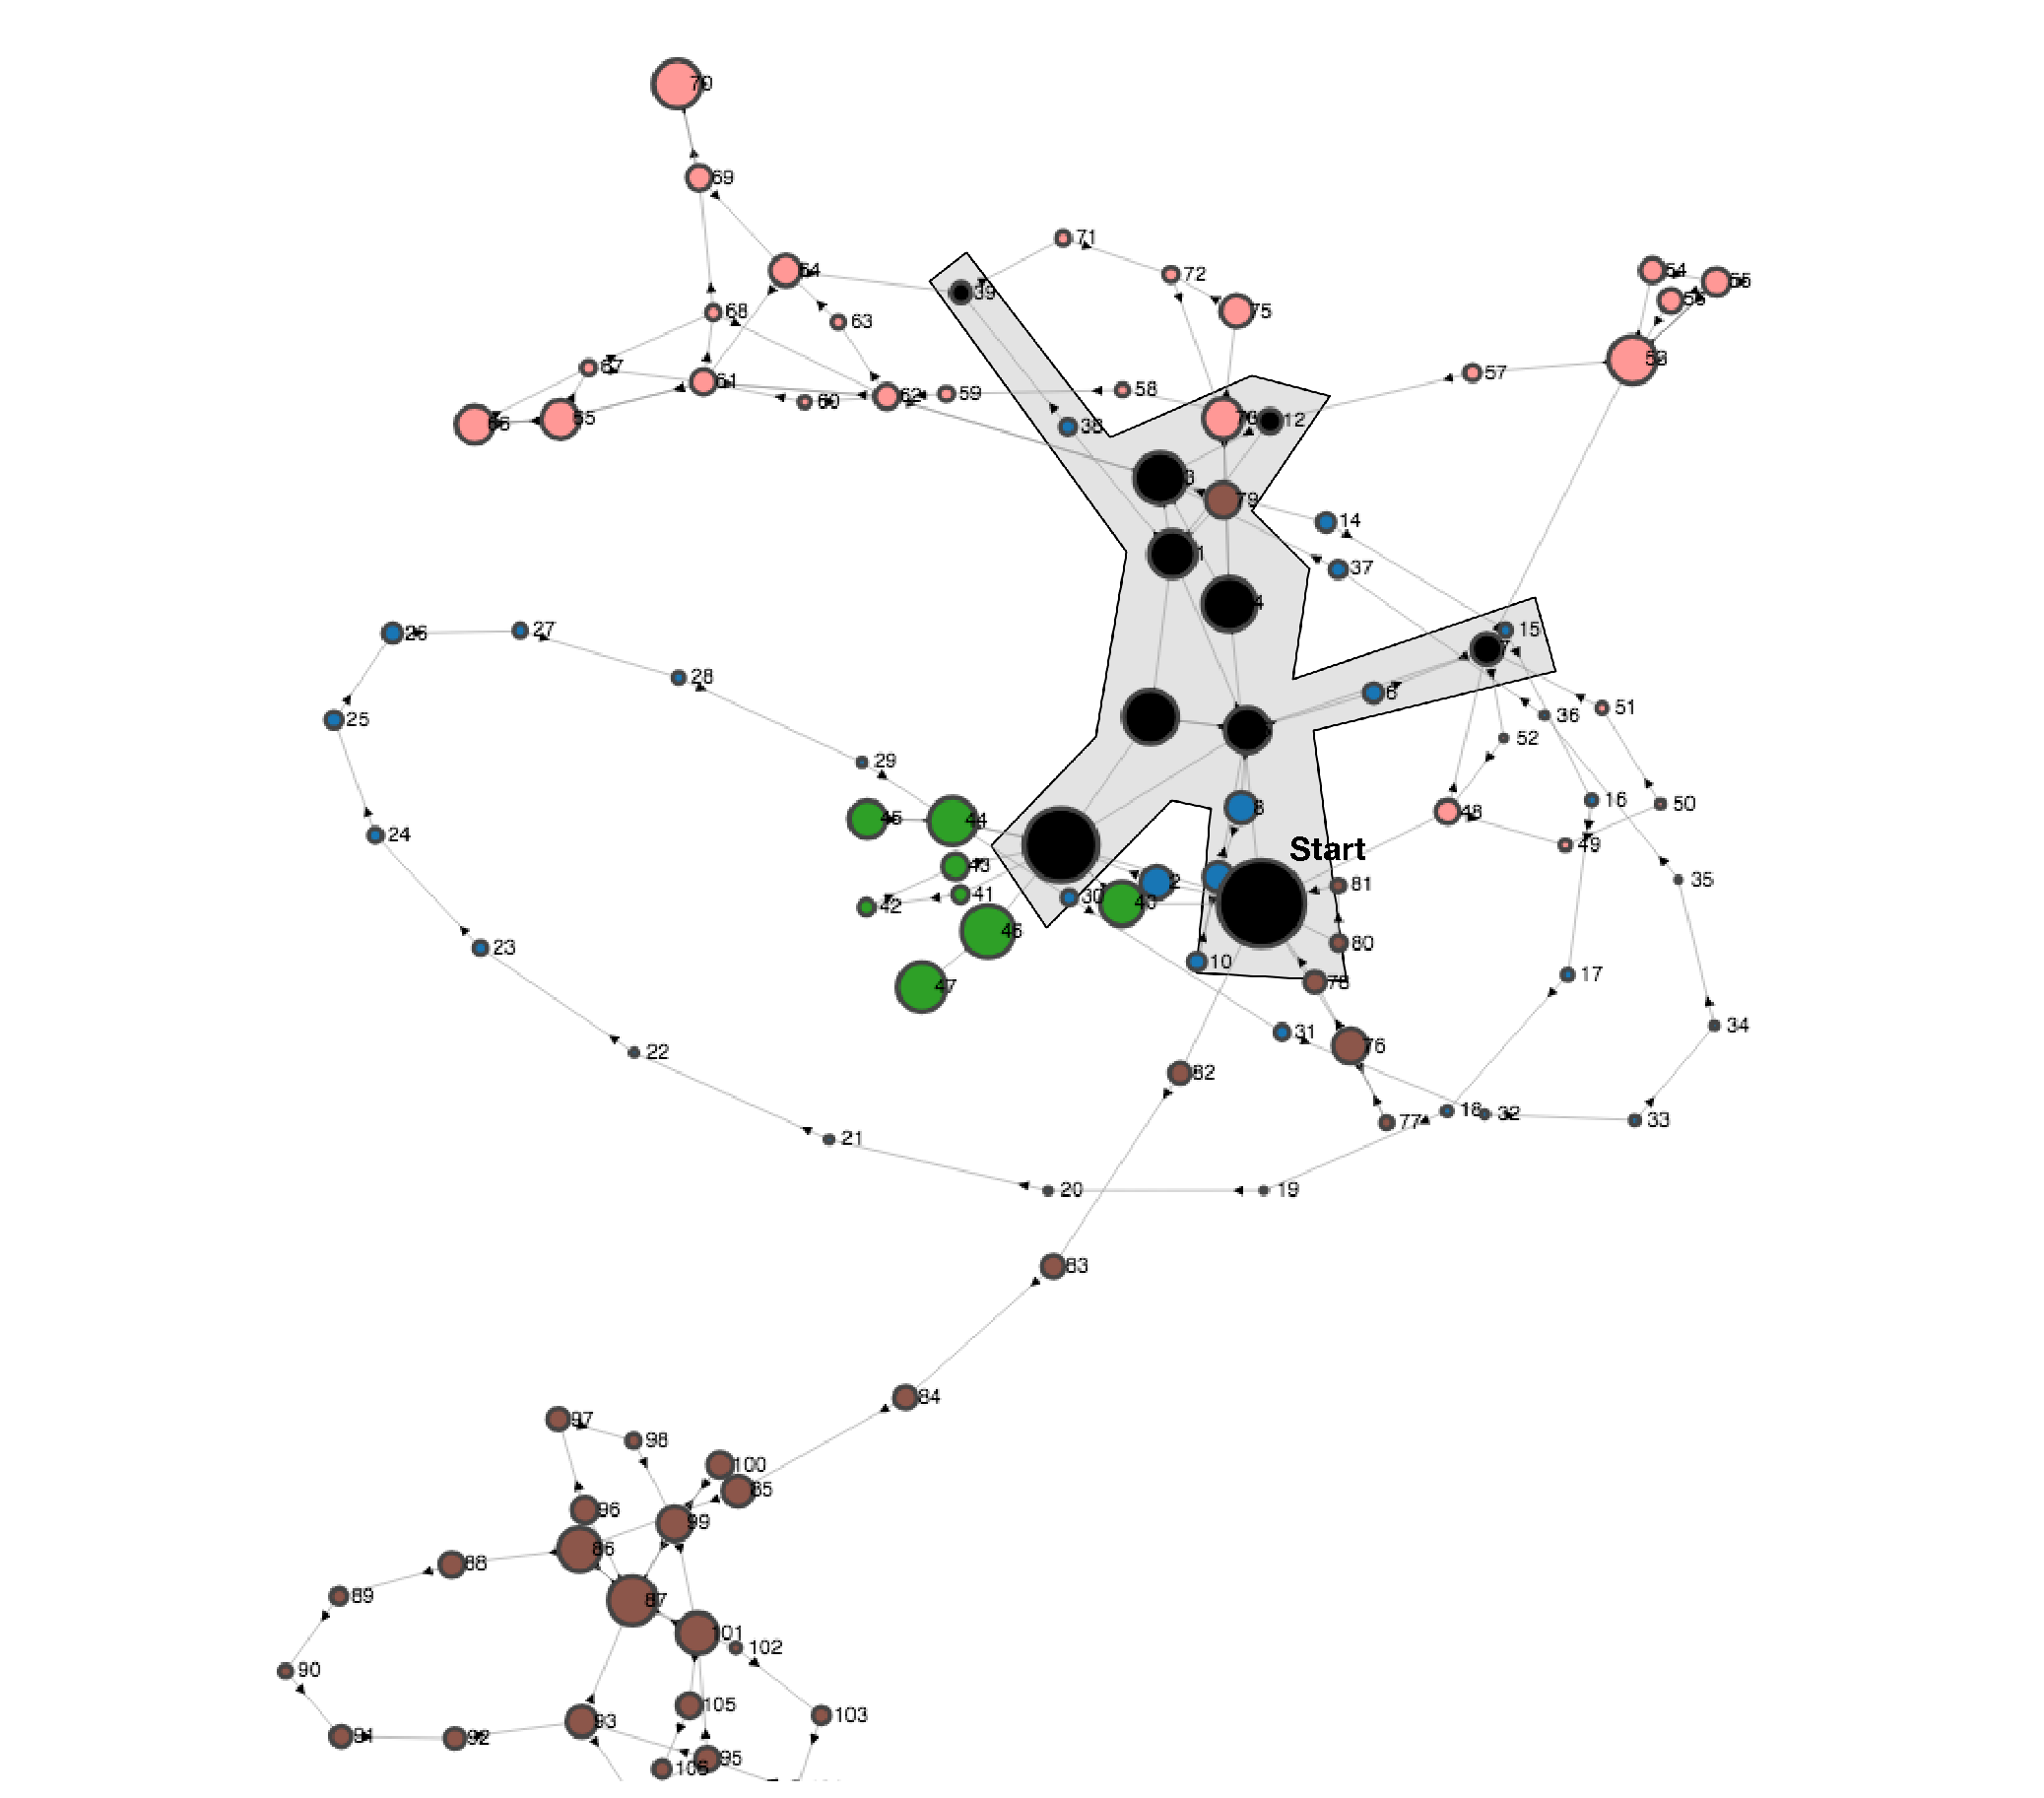
\includegraphics[width=1\textwidth]{figures/overlap1}
        \caption{Example of ``overlap'' pattern: this figure visualize the clickstream intersection 
        of four participants at Medium's goal-oriented task. Each color represents an
        individual clickstream except black nodes, which represents the overlapping of different clickstreams.
        The overlap ratio of this graph is 9.43\%.}
        \label{fig:overlap-example-1}
    \end{subfigure}

    \begin{subfigure}[b]{0.60\textwidth}
        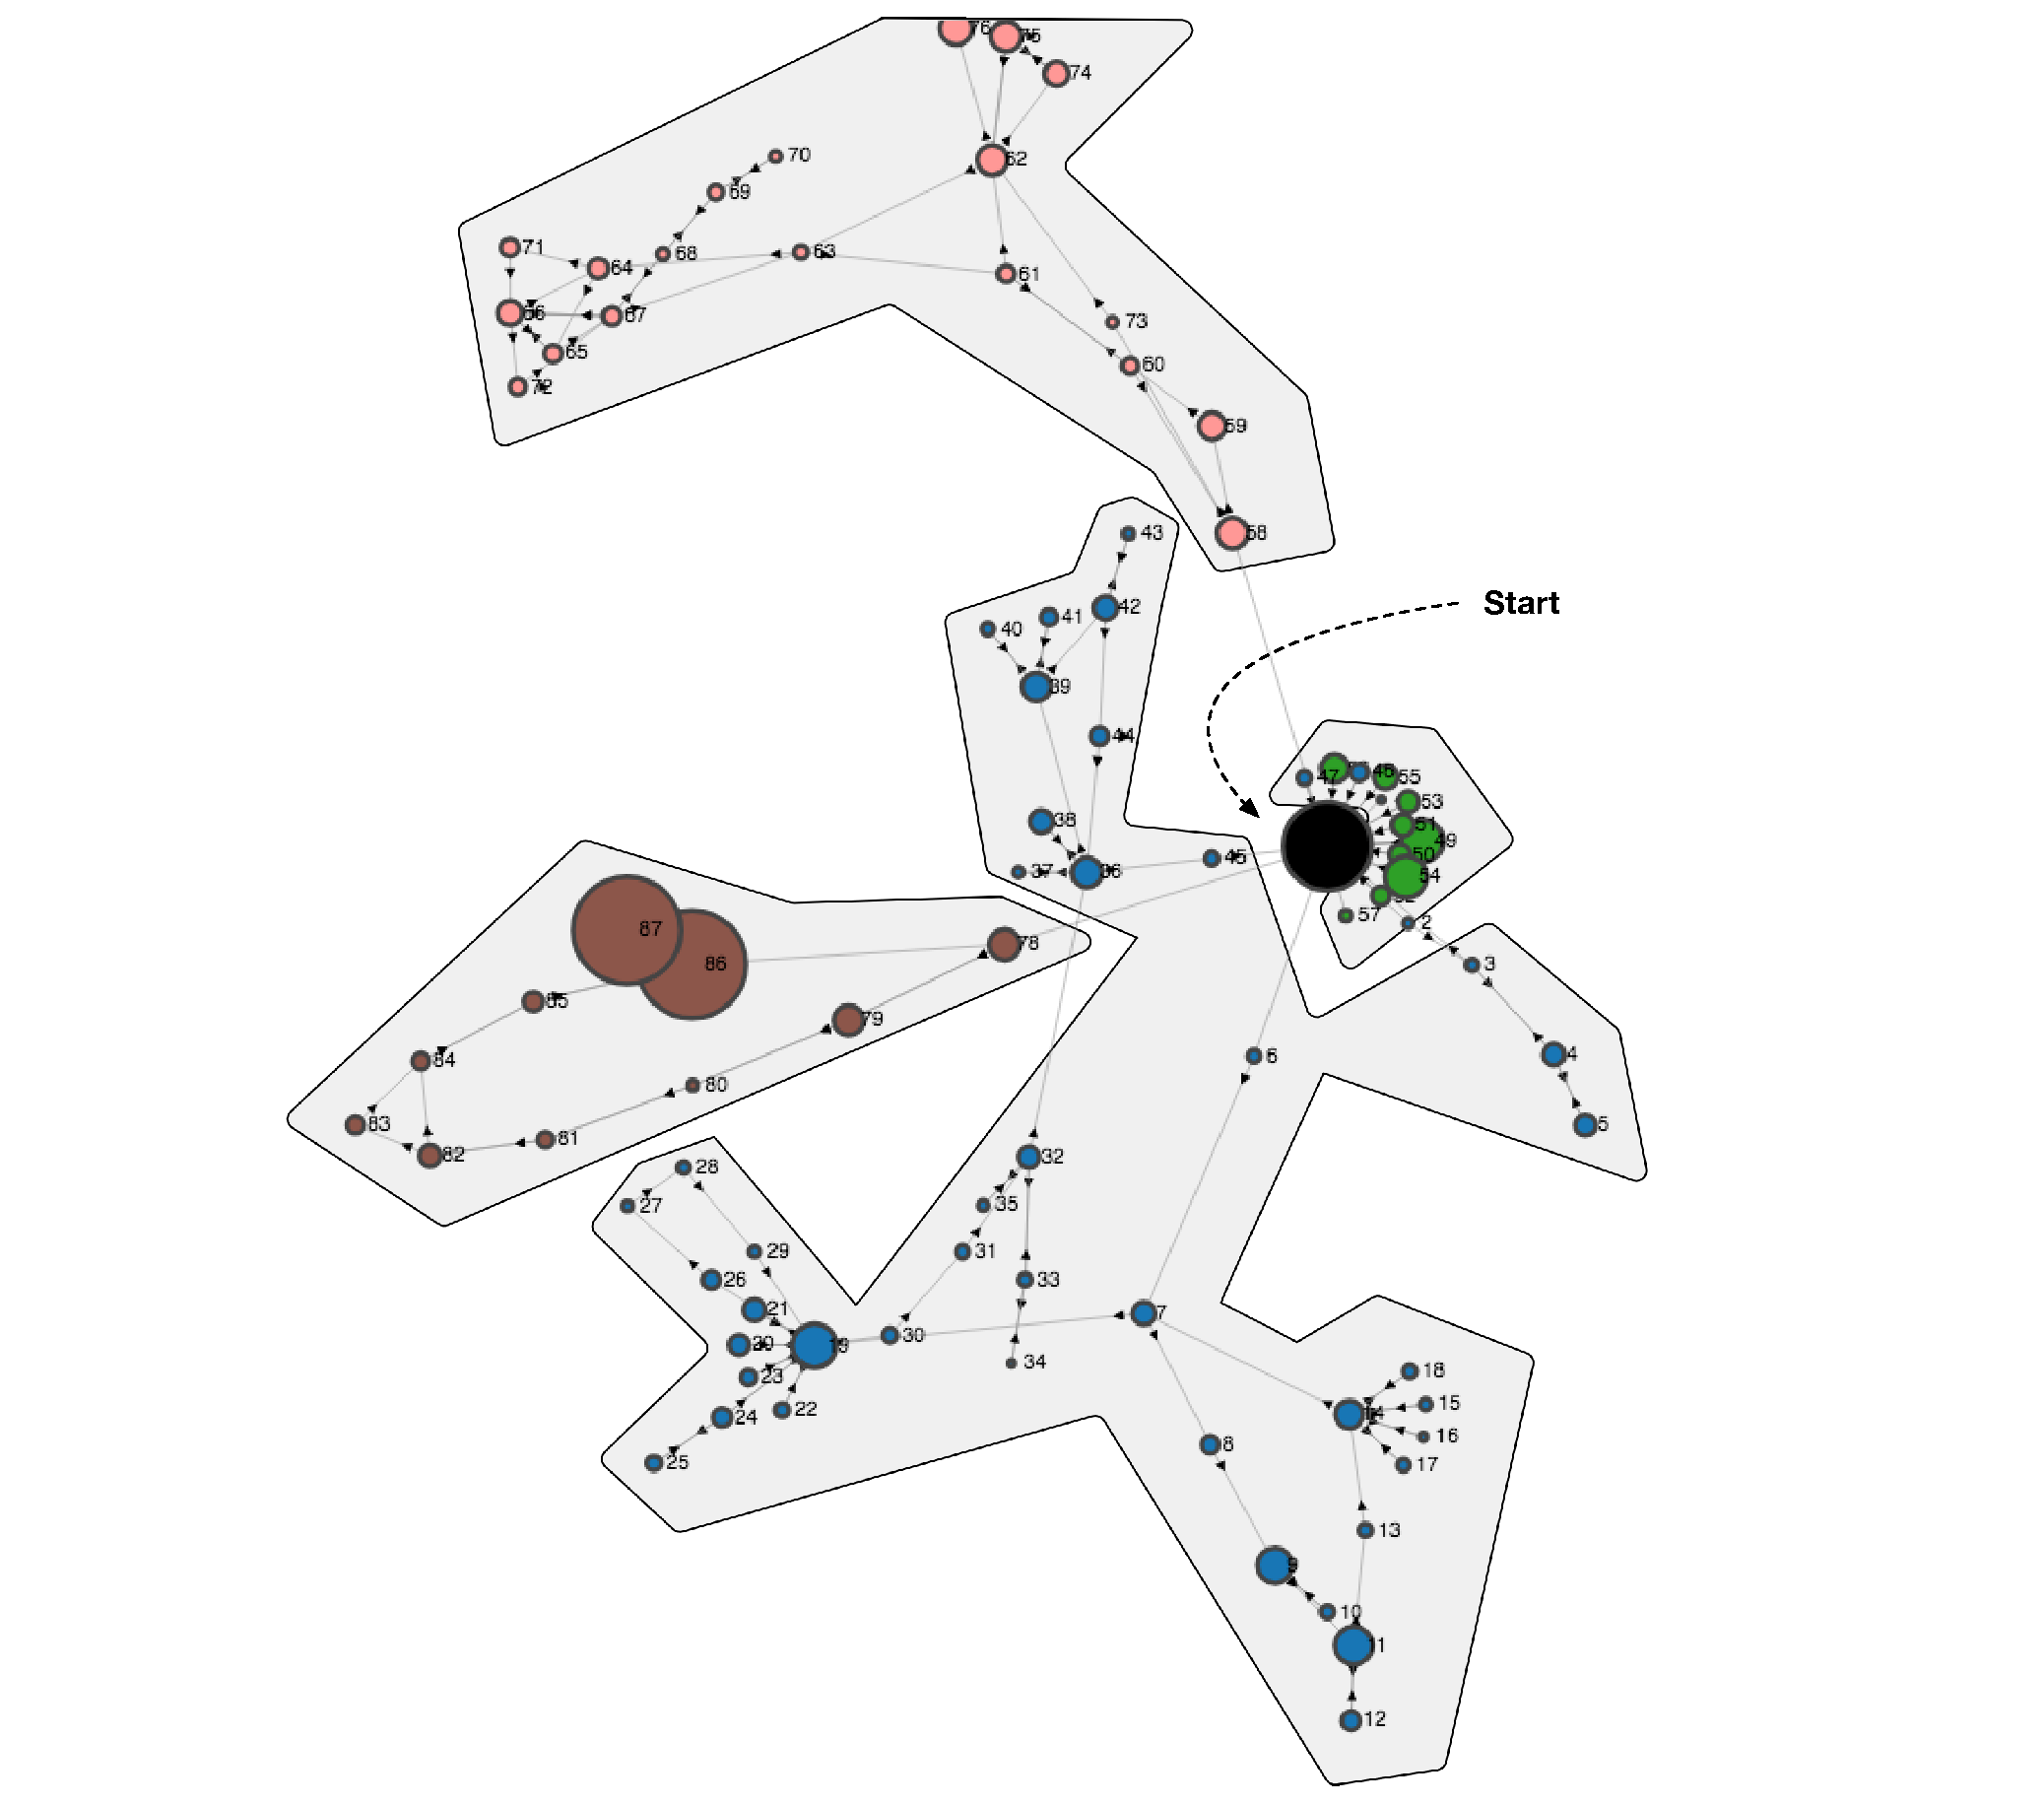
\includegraphics[width=1\textwidth]{figures/overlap2}
        \caption{Example of ``overlap'' pattern: this fugure visualize the clickstream intersection
        of four participants at Dribbble's exploring task. Each color represents an
        individual clickstream except blacken nodes, which represents the overlapping of different clickstreams.
        The overlap ratio of this graph is 1.15\%.}
        \label{fig:overlap-example-1}
    \end{subfigure}

    \caption{Example of ``overlap'' pattern: In this two figures, the raw clickstreams in
    Medium's goal-oriented task and Dribbble's exploring task are vidualized
    for same four participants, which intent to compare and analysis for two type of browsing behavior.
    Blacken nodes represent the overlap of different clickstreams, and the highest overlap ratio
    in our dataset is 11.84\% and lowest overlap ratio is 0.00\%. Besides, the number of a node
    is a representative of chronological serial number of user actions.
    }
    \label{fig:overlap-examples}
\end{figure}

\paragraph{Remark}

\begin{table}[H]
    \small
    \centering
    \caption{Existence of activities from Ellis' Model and information use in the observed patterns}
    \begin{adjustbox}{width=\textwidth}
        \begin{tabular}{ccccccccc}
            \toprule
            \multicolumn{1}{c}{\multirow{2}{*}{\textbf{Behaviors}}}  & \multicolumn{1}{c}{\multirow{2}{*}{\textbf{Information Need}}} & \multicolumn{6}{c}{\textbf{Information Seeking}}                                    & \multicolumn{1}{c}{\multirow{2}{*}{\textbf{Information Use}}} \\ \cline{3-8}
            \multicolumn{1}{c}{}                                     & \multicolumn{1}{c}{}                                  & \textbf{Starting} & \textbf{Chaining} & \textbf{Browsing} & \textbf{Differentiating} & \textbf{Monitoring} & \textbf{Extracting} & \multicolumn{1}{c}{}  \\
            \hline
            cluster    &   observed &       &       &       & Exist & Exist & Exist & Exist \\
            star       &            &       & Exist & Exist & Exist &       &       &       \\
            ring       &            & Exist & Exist &       &       &       &       &       \\
            hesitation &   observed &       &       &       & Exist & Exist &       &       \\
            overlap    &   observed &       &       &       &       &       & Exist & Exist \\
            \bottomrule
        \end{tabular}
        \label{table:ellis}
    \end{adjustbox}
\end{table}

\cleardoublepage